\chapter{Einführung}
\label{Einfuehrung}

\section{Nutzen und Erwartungen}
\label{Nutzen}

Lineare Baumstrukturen entstehen oft durch lineare Blockabhängigkeiten. Diese Abhängigkeiten sind jedoch oft nicht zwingend linear, sonder werden der Einfachheit halber vom Compiler so dargestellt. Beispiele hierfür finden sich oft in verschachtelten Strukturen von algebraischen Relationen. \\
Die folgende Rechnung \ref{eq:beispiel-addition} wird oft mit einem rechts- oder links-assoziativen Abhängigkeitsgraph abgebildet. Dies führt dazu, dass in Mehrkernsystem die einzelnen Operationen nicht parallel durchgeführt werden können.

\begin{equation} \label{eq:beispiel-addition}
a + b + c + d + e + f + g + h
\end{equation}

In einer links-assoziativen Baumstruktur (siehe Abbildung \ref{fig:links-assoziativer-baum}) ist ein linearer Programmfluss vorgegeben. Jeder Schritt baut hierbei auf die vorherige Operation auf. In Tabelle \ref{tab:links-assoziativer-baum} sind die Befehle aufgelistet, welche aus dem links-assoziativen Baum in Abbildung \ref{fig:links-assoziativer-baum} folgen. Die Befehle sollen hierbei für einem 2-Kern-System optimiert werden. Die Bezeichner \textit{t1} bis \textit{t7} stehen dabei für die einzelnen Teilbäume, beziehungsweise ihre Zwischenergebnisse. Wie zu sehen werden die Befehle nur auf einen Kern ausgeführt. Der andere Kern kann nicht agieren, da ihm immer eine Abhängigkeit zum Folgebefehl fehlt.\\

Wünschenswert wäre an dieser Stelle jedoch ein Befehlssatz, welcher auf Mehrkernsystemen (zum Teil) parallel ausgeführt werden kann. Dadurch könnten Prozessortakte und somit die Laufzeit des kompilierten Programmes eingespart werden.\\
Das Verfahren des Tree-Height-Balancing soll hierbei angewendet werden, um die links- oder rechts-assoziativen Bäume auszubalancieren. Sofern die Kinder eines Baumes nicht untereinander Abhängigkeiten aufweisen, können diese parallel vom Prozessor bearbeitet werden. Die führt zur Ausführung vom mehreren Befehlen innerhalb eines Taktes in Mehrkernsystemen.


\begin{figure}
	\begin{center}
	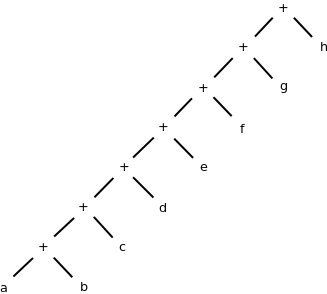
\includegraphics[width=0.5\textwidth]{images/links_assoziativer_baum}\\
	\end{center}
	\caption{Links-assoziativer Baum}
	\label{fig:links-assoziativer-baum}
\end{figure}

\begin{table}
	\begin{center}
			\begin{tabular}{|c|c|c|}
				\hline  & Kern 1 & Kern 2 \\ 
				\hline 1 & $ t1 \leftarrow a + b $& - \\ 
				\hline 2 & $ t2 \leftarrow t1 + c $& - \\ 
				\hline 3 & $ t3 \leftarrow t2 + d $& - \\ 
				\hline 4 & $ t4 \leftarrow t3 + e $& - \\ 
				\hline 5 & $ t5 \leftarrow t4 + f $& - \\ 
				\hline 6 & $ t6 \leftarrow t5 + g $& - \\ 
				\hline 7 & $ t7 \leftarrow t6 + h $& - \\ 
				\hline 
			\end{tabular}
	\end{center}
	\caption{Befehle für links-assoziativen Baum}
	\label{tab:links-assoziativer-baum}
\end{table}

\newpage
\section{Dependency Graph als Einstiegspunkt}
\begin{quotation}
"'Compilers also use graphs to encode the flow of values from the point where a value is created, a definition, to any point where it is used, a use. A data-dependency graph embodies this relationship." \cite{HeBIS-309344573}
\end{quotation}
Ein Abhängigkeitsgraph (dependency graph) stellt den Informationsfluss zwischen den Attributinstanzen eines bestimmten Parse-Baumes dar. Eine Kante von einer Attributinstanz zu einer anderen bedeutet, dass der Wert der ersten benötigt wird, um den der zweiten zu brechnen. Kanten drücken die durch die semantische Regeln auferlegten Einschrängungen aus. "'Für jeden \textbf{Knoten} des Parse-Baumes, der mit dem Grammatiksymbol X bezeichnet sei, weist der Abhängigkeitsgraph für jedes mit X verbundene Attribut einen Knoten auf. Angenommen, eine mit einer Produktion p verbundene semantische Regel definiert den Wert des synthetisierten Attributes A.b durch den Wert X.c . Dann hat der Abhängigkeitsgraph eine \textbf{Kante} von X.c nach A.b . \cite{HeBIS-194410269}"' 

Der Algorithmus verlangt einen Abhängigkeitsgraphen, der in der ersten Phase bearbeitet wird. Zur Erstellung eines Abhängigkeitsgraphen bedarf es den Vorstufen des Compilers. Um es kurz zu halten: Ein Scanner muss die Tokens mit Hilfe von regulären Ausdrücken einlesen und ein Parser diese in einen Parse-Baum wandeln. Aufgrund zeitlicher Begrenzung und der durch den Algorithmus gegebenen Komplexität, wird ein Abhängigkeitsgraph manuel erstellt. Dieser Ablauf wird im folgenden näher erklärt.

\subsection{Graph - Linked Implementation} 
Ein Graph ist eine Datenstruktur, in der Informationen gespeichert werden können. Im Gegensatz zu Bäumen, die eine hierarchische Struktur besitzen, sind Graphen flexibler. Die Konsequenz daraus ist, dass Graphen auch Schleifen haben können und ein Knoten in einem Graphen nicht unbedingt erreichbar sein muss (siehe Abbildung \ref{fig:Graph}).
\begin{figure}[h]
\centering
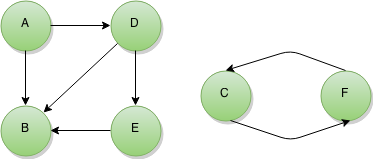
\includegraphics[scale=0.5]{images/Graph.png} 
\caption{Beispiel eines Graphen.}
\label{fig:Graph}
\end{figure}
Wie in Abbildung \ref{fig:Graph} zu sehen ist, besteht der Graph aus den Knoten A, B, C, D, E und F. Diese Knoten werden auch \textit{vertices} oder auch \textit{vertex} bezeichnet. Knoten können, müssen aber nicht, mit einander verbunden sein. Eine Verbindung zwischen zwei Knoten wird als Kante oder auch \textit{edge} definiert und wird grafisch durch die gerichteten Pfeile dargestellt. Die Informationen sind in den jeweiligen Knoten gespeichert und werden durch die Kanten in Abhängigkeit gesetzt. 

\subsubsection*{Darstellung in C}
Ein Graph wird oft mit Hilfe einer \textit{Adjazenzmatrix\footnote{Wird auch Nachbarschaftsmatrix genannt}} oder einer \textit{Adjazenzliste} abgebildet. Eine Adjazenzmatrix ist eine 2D N x N Matrix, wobei N die Einträge der Knoten des Graphen sind. Die Matrix wird so aufgebaut, dass eine Verbindung zwischen zwei Knoten mit einer \textbf{1} versehen werden. Alle anderen Felder sind mit einer \textbf{0} gekennzeichnet. Dies hat Zufolge, dass viel Speicherplatz dadurch verbraucht wird, indem die unrelevante Information (keine Verbindung) ebenfalls dargestellt wird. Des Weiteren muss die Größe des Arrays bekannt sein. 

Abhilfe schafft hier die Adjazenzliste. Diese Liste kann mit einer "'Linked List"' in C abgebildet werden. Dabei spielt die Anzahl der Knoten keine Rolle und wird nur durch den pyhsikalischen Speicher begrenzt. Abbildung \ref{fig:adjacencelist} zeigt den Graphen in einer Adjazenzliste. Ein Eintrag in der vertikalen Liste beinhaltet jeweils einen Knoten des Graphen und hat ein Verweis auf deren Nachfolger. Jeder Knoten speichert seine Verbindungen, also Kanten, ab. 
\begin{figure}[h]
\centering
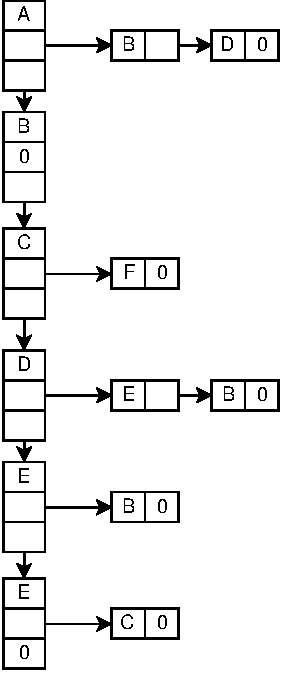
\includegraphics[scale=0.85]{images/adjacencelist.pdf} 
\caption{Adjazenzliste des Beispiel-Graphen.}
\label{fig:adjacencelist}
\end{figure}
Eine Implementation einer Adjazenzliste ist im Listing \ref{list:graph} abgelegt. Die vertikale Liste ist die \textit{vertex - Liste} und die horizontale Liste ist die \textit{edege - Liste}. Das Element \textit{connectTo} ist ein Pointer auf ein Vertex. Dadurch werden Kanten zwischen den Knoten definiert. Es wird also kein neuer Knoten angelegt, sondern auf einen der im Graphen enthalten ist, verwiesen. Ein Abhängigkeitsgraph speichert einen Graphen und eine Liste, der im Graphen befindlichen Variablen (UEVARS), ab.
\begin{lstlisting}[caption=Struktur eines Graphen., label=list:graph]
typedef struct vertexTag {
  char* element;    
  char* operation;  
  int isConstant;
  int isVisited;
  struct edgeTag* edge;
  struct vertexTag *next;
} vertex;

typedef struct edgeTag {
    struct vertexTag *connectsTo;
    struct edgeTag *next;
 } edge;

typedef struct graphTag{
  vertex *vertices;
}graph;
\end{lstlisting}

\subsubsection*{Estellung von Abhängigkeitsgraphen}
Zur Erstellung eines Abhängigkeitsgraphen werden Datein mit der Endung "'.depg"' angelegt. Dadurch wird es Möglich eine große Anzahl von Graphen zu erstellen und den Algorithmus auszutesten. Dafür wurde eine Syntax gewählt, die die Knoten, Kanten und Variablen, welche aus einem anderen Block kommen, des Graphen definieren. Dabei ist die Eingabe der Reihenfolge von Wichtigkeit, da ansonsten Zugriffsfehler enstehen können. Es wird verlangt, dass die Knoten zuerst definiert werden und somit die vertikale Struktur beschrieben werden kann. Dabei wird die Definition der Knoten mit \textit{vertex:} eingeleitet und mit einem Komma separiert. Der jeweilige Knoten ist durch Brackets ("'["' , "']"') umschlossen. Hinter der Angabe des Knotennamens folgt die definition des Knotentypes. 
\begin{lstlisting}[caption=Konstruktion eines Abhängigkeitsgraphen., label=list:dg]
vertex: [y(+)],[z(*)],[t1(*)],[t2(-)],[a(const)],[b(const)],[c(const)]
edge:   [y->t1] , [z->t1] , [y->t2] , [z->t2] , [t1->a] , [t1->b] ,[t2->c] 
uevar:  [a],[b],[c],[d]
\end{lstlisting}
Ähnlich werden die Verbindungen der Knoten konstruiert. Eingehend mit dem Akronym \textit{edge:} werden die Kanten mit einem Komma getrennt eingelesen. Eingeklammert in Backets werden zwei Knoten durch einen Pfeil definiert (siehe Listing \ref{list:dg}). 

Jeder Abhängigketsgraph speichert eine Liste von Variablen, die außerhalb des Blockes definiert wurden. Das 
vorangehende \textit{uevar:} leitet eine Liste, die ebenfalls durch Kommas getrennt ist, von Variablen ein. Jede Dekleration wird mit einem Carriage return abgeschlossen.

